\chapter{Introduction}\label{Chap:Introduction}

\section{Samples}
In this section, a number of short examples how to use the packages will be given.

\subsection{Citations and References}\label{SubSec:Citations}
Citations can be easily made by the \textbackslash cite-command. At first, prepare your literature database in the literature.bib-file. Then simply use the cite-command and the bibtex-key to cite the desired original source. The bib-file can be either exported from literature managing software like Citavi or EndNote (consult your manual) or you directly use the bib-file for your literature database (in this case we recommend you to use JabRef for having a nice front-end instead of editing the text files).

References to other items (figures, tables, equations, sections, subsections and so on...) can either be made with \textbackslash ref or \textbackslash autoref. While for the first command you have to provide the type of item (like see Chapter~\ref{Chap:Introduction}), the \textbackslash autoref-command takes care of using the right label (\autoref{SubSec:Citations}). One last remark on references and citations: Use a non-breaking space between the element you refer on and the citation/reference. This can be achieved by using a tilde character (\textasciitilde) instead of a blank between the elements. Otherwise \LaTeX is allowed to insert a line break between the both.

\subsection{Figures}
You can include any kind of graphics (tif,bmp, png,jpg,pdf,eps) in your thesis as a figure. Some small notes:
\begin{itemize}
	\item Always try to use the CMYK color model whenever possible. When printing your thesis the printer will work with this color model. It will make a huge difference for the colors you used in your thesis between computer screen and printout!
	\item When using jpg's, make sure to export them in high quality mode. Otherwise you will experience a gray blur around your figures because of too strong compression.
	\item When using pngs keep in mind that png uses its own color model for display on a computer display. If you want to print your thesis, the colors will not be the same (CMYK color model on printers). This means, png is perfectly fine for gray-scale figures, but try to avoid it for colored ones.
	\item Vector graphics (pdf, eps) are best suited for rescaling them in \LaTeX. If you have to use raster-based formats (tif, bmp, png, jpg), make sure the resolution of the image is large enough and that you do not change the aspect ratio of the original image.
\end{itemize}

\autoref{Fig:SampleFig1} is a sample of how to embed a graphic file into your thesis. Try to place you figures always at the top or the bottom of a page. Never embed a figure, table or plot between paragraphs!

\begin{figure}
	\centering
	
\includegraphics[width=0.5\textwidth]{Figures/TUM_Logo_cmyk.pdf}
	\caption{Sample figure (some kind of famous logo).}
	\label{Fig:SampleFig1}
\end{figure}
\newpage

\subsection{Tables}
\autoref{Tab:TableTest} gives an example of how to use tables. The caption has to be above the table. You can define different types of column alignment (l=left, c=center, r=right, S=for numbers). Please see the effect of the different types in the following table. The S-column is a special column provided by the siunitx package for typesetting numbers in tables. These are aligned on the decimal point rather than the total length of the number. This is especially useful if you encouter different number of significant digits. Text in an S-column has to be wrapped in curly brackets (\{\}).

One word about constructing a table: Try to avoid vertical lines whenever possible, they often interrupt the normal reading flow from left to right. The booktabs-package provides you with thicker lines for the first and last lines of a table (\textbackslash toprule and \textbackslash bottomrule). Have a look at the example.

\begin{table}
	\caption{Table for testing.}
	\label{Tab:TableTest}
	\centering
	\begin{tabular}{lcrS}
		\toprule
		Header		& Center			& New Column	& $\rho$ in $\si{\kg \per \meter^3}$ \\
		\midrule
		Row 1		& Cell 2			& 2.5553		& 2.5553 \\
		Row 2		& 123				& 235.2			& 235.2  \\
					& First was empty	& ABC			& {TEXT} \\
		\bottomrule
	\end{tabular}
\end{table}

\subsection{siunitx}
The package siunitx helps you to typeset SI-units correctly. Please always keep in mind, that while symbols are always in itallic font, units are typesetted in normal font (see \url{http://physics.nist.gov/cuu/pdf/checklist.pdf}) It can either by used in normal text to give quantities, for example \SI{1.3}{\kg \per \meter^3}, or just units, like \si{\micro \N / \square \meter}. Please refer to the documentation for further options and possibilities (\url{http://ctan.mackichan.com/macros/latex/contrib/siunitx/siunitx.pdf}). siunitx can also be used in math mode:

Example 1:\quad $c_{p}\left(Water\right) = \SI{4.2}{\J \per \kg \K}$\\
Example 2:
\begin{align}
	P_{el} = \SI{3}{\mega \watt}
\end{align}

When giving equations, either use quantity equations, that are independent of the measurement unit, like
\begin{align}
	\Reyn = \frac{\rho \cdot d \cdot u}{\eta},
\end{align}
where the units of both sides of the equation are equal (in this case dimensionless), or use numerical value equations:
\begin{align}
	\frac{\dot{V}}
		 {\left[\si{\liter \per \second}\right]} 
		= -1 + 2.247 \cdot \exp{\left(
							0.04266\cdot
							\frac{h}{\left[ \% \right]}
							\right)}
\end{align}
Here, you explicitly have to give all units of the involved numerical quantities. This means, the equation is only valid for the given set of units (e.g. useful for fitted equations without physical background) and the user of the equation has to take care of doing the unit conversion before using the equation. Never give the units needed for such an equation in the text, always clearly state them in the equation itself. Further information can be found in the ISO~80000-1~\cite{ISO80000}.

\subsection{Plotting}
TIKZ and pgfplots can be used to do plotting inside \LaTeX. In the following some samples of how to plot data are given. If you need any special functionality, always check both documentations first (\url{ftp://ftp.mpi-sb.mpg.de/pub/tex/mirror/ftp.dante.de/pub/tex/graphics/pgf/base/doc/pgfmanual.pdf} and \url{http://pgfplots.sourceforge.net/pgfplots.pdf}).

pgfplots can be used to plot data from equations provided, like the polynomials in~\autoref{Fig:SampleFigPoly}. Other examples are subplots (see~\autoref{Fig:Theo_SFDev}, where you can refer to one subfigure as well~\autoref{Fig:Sample_Subfig1}) or the plotting from an external csv-file (\autoref{Fig:Intro_Occurences}).

Always try to make your plots as simple and distinct as possible. Do not use the same type of line for all data series. When employing colors (try to avoid them when possible), make sure the plot can be copied in grayscale mode so that the elements are still clearly distinguishable. If different line types are not enough and you have to use colors, it may be better to distribute the data to two separate graphs.

\begin{figure}
	\centering
	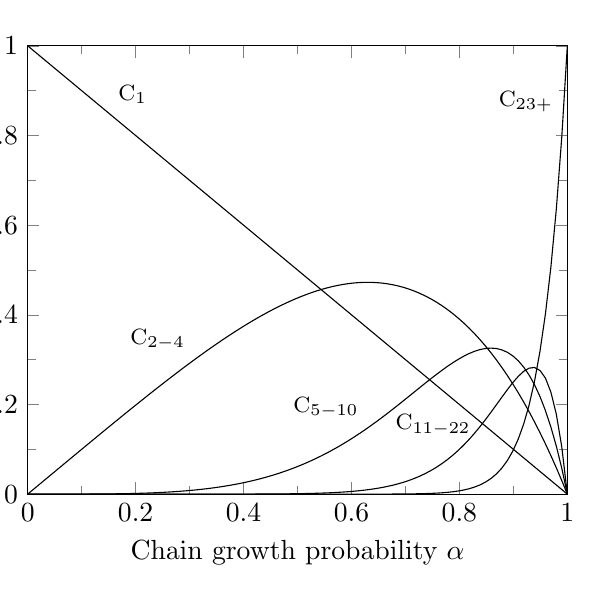
\begin{tikzpicture}[trim axis left]
	\begin{axis}[
	xlabel=Chain growth probability $\alpha$,
	ylabel=Molar fraction $x_n$,
	ymin=0, ymax=1,
	xmin=0, xmax=1,
	minor tick num=1]
	\addplot[domain=0:1, samples = 100]{(1-x)} node [pos=0.15,font=\footnotesize,anchor=south west] {$\mathrm{C}_{1}$};
	\addplot[domain=0:1, samples = 100]{(1-x)* (x+x^2 + x^3)} node[pos=0.3,font=\footnotesize,anchor=south east] {$\mathrm{C}_{2-4}$};
	\addplot[domain=0:1, samples = 100]{(1-x)*(x^4 + x^5 + x^6 + x^7 + x^8 + x^9)}  node[pos=0.5,font=\footnotesize,anchor=south east] {$\mathrm{C}_{5-10}$};
	\addplot[domain=0:1, samples = 100]{(1-x)*(x^10 + x^11 + x^12 + x^13 + x^14 + x^15 + x^16 + x^17 + x^18 + x^19+x^20+x^21)}  node[pos=0.62,font=\footnotesize,anchor=south east,xshift=6] {$\mathrm{C}_{11-22}$};
	\addplot[domain=0:1, samples = 100]{1-((1-x)*(1 + x   + x^2 +x^3 + x^4 + x^5 + x^6 + x^7 + x^8 + x^9 + x^10 + x^11 + x^12 + x^13 + x^14 + x^15 + x^16 + x^17 + x^18 + x^19+x^20+x^21))}  node[pos=0.91,font=\footnotesize,anchor=south east] {$\mathrm{C}_{23+}$};
	\end{axis}
	\end{tikzpicture}
	\caption{ASF hydrocarbon product distribution. Sample plot of how to use polynomials for plotting data.}
	\label{Fig:SampleFigPoly}
\end{figure}

\begin{figure}
	\centering
	\begin{subfigure}[b]{.49\linewidth}
		\resizebox{\linewidth}{!}{
			\begin{tikzpicture}
			\begin{axis}[
			xlabel=Chain length,
			ylabel=Molar fraction $x_n$,
			ymin=0.001, ymax=0.3,
			xmin=0,
			ymode = log,
			enlarge x limits=false]
			\addplot[color=black,solid, mark=none] table [x=n, y=x1, col sep = semicolon] {Data/SFPlot.csv};
			\end{axis}
			\end{tikzpicture}}
		\caption{Note the semilogarithmic axes.}
		\label{Fig:Sample_Subfig1}
	\end{subfigure}
	\begin{subfigure}[b]{.49\linewidth}
		\resizebox{\linewidth}{!}{
			\begin{tikzpicture}
			\begin{axis}[
			xlabel=Chain length,
			ylabel=Molar fraction $x_n$,
			ymin=0.001, ymax=0.3,
			xmin=0,
			ymode = log,
			enlarge x limits=false]
			\addplot[color=black,solid, mark=none] table [x=n2, y=x2, col sep = semicolon] {Data/SFPlot.csv}
			node  [pos=0.2,anchor=south west] {$\alpha_{1}$}
			node  [pos=0.7,anchor=south west] {$\alpha_{2}$};
			\end{axis}
			\end{tikzpicture}
		}
		\caption{Two chain growth probabilities.}
		\label{Fig:Sample_Subfig2}
	\end{subfigure}
	\caption{Sample of how to use subfigures.}
	\label{Fig:Theo_SFDev}
\end{figure}

\begin{figure}
	\centering
	\begin{tikzpicture}
		\begin{axis}[
			width=0.8\textwidth,
			height=0.50\textwidth,
			axis y line* = left,
			ylabel = Relative frequency,
			xlabel = Year,
			ymin = 0,
			ymax = 3.0e-5,
			xmin = 1925,
			xmax = 2006,
			/pgf/number format/.cd,
			1000 sep={},]
			\addplot [color=black,solid, mark=none] table [x=Year, y=FT, col sep = comma] {Data/ngram.csv}; \label{Plot:t_FT}
			\addplot [color=black,dash dot, mark=none] table [x=Year, y=Sasol, col sep = comma] {Data/ngram.csv};\label{Plot:t_Sasol}
			\addplot [color=black,dashed, mark=none] table [x=Year, y=Farben, col sep = comma] {Data/ngram.csv};\label{Plot:t_Farben}
		\end{axis}
		\begin{axis}[
			width=0.8\textwidth,
			height=0.5\textwidth,
			axis y line* = right,
			axis x line = none,
			ylabel = Crude oil price in $\si{\$ \per bbl}$,
			ymin = 0,
			ymax = 60,
			xmin = 1925,
			xmax = 2006,
			legend pos = north west,
			legend cell align=left,
			legend style = {font=\scriptsize}]
			\addlegendimage{/pgfplots/refstyle=Plot:t_FT}
			\addlegendentry{Fischer-Tropsch}
			\addlegendimage{/pgfplots/refstyle=Plot:t_Sasol}
			\addlegendentry{Sasol}
			\addlegendimage{/pgfplots/refstyle=Plot:t_Farben}
			\addlegendentry{I.G. Farben}
			\addplot [color=red,solid, mark=none] table [x=Year, y=Oil, col sep = comma] {Data/ngram.csv};
			\addlegendentry{Crude Oil Price}
		\end{axis}
	\end{tikzpicture}
	\caption[Short title for table of figures summary.]
	{Long title. Sample plot for showing how to plot data from a csv-File on two y-Axis and a lot of customization}
	\label{Fig:Intro_Occurences}
\end{figure}
\newpage

\subsection{Final Note}
If you encounter some problems during writing your thesis with \LaTeX (and you will!), it is always a good idea to comment out specific parts and try to recompile your document. Step-by-step you will find out what the error is (most often: missing brackets).

A good source for information on how to use the packages, how to modify the options and which additional functionality is provided are the official documentations of the corresponding packages. Most often they are well written with numerous copy-and-paste samples.

\url{http://tex.stackexchange.com/} is a very good source for finding relevant information concerning error messages, problems while typesetting your document and examples. If you do not know any further with your problem, try to assemble a minimal working example (MWE) and post it there. The people there are very friendly and have a lot of expertise with \LaTeX, which they are happy to share. Never try to post a full document or without code, as the people there will not be able or willing to help you.